\documentclass[12pt, a4paper]{article}
% --- 基础宏包 ---
\usepackage[UTF8]{ctex}     % 中文支持
\usepackage{geometry}       % 页面布局
\usepackage{hyperref}       % 超链接支持
\usepackage{natbib}
\usepackage{booktabs}
\usepackage{newtxtext}      
\usepackage{newtxmath}      
\usepackage{multicol}
\usepackage{multirow}
\usepackage{bm}
\usepackage[numbers,super]{natbib}

\usepackage{amssymb}

\usepackage{algorithm}
%\usepackage{algorithmic}
\usepackage{algpseudocode}
\usepackage{graphicx}
\usepackage{subfig}
\usepackage{float}
\usepackage{amsmath}
% --- 页面设置 ---
\geometry{left=1in, right=1in, top=1in, bottom=1in}
% --- 标题信息 ---
\title{\textbf{网约车个体补贴分配问题的数学建模}}
\begin{document}
% 标量用默认字体
% 向量用 \bm
% 集合用大写字母
% 向量集合用 \mathcal
\maketitle

\section{符号说明}
全文所用数学符号定义如表~\ref{tab:nomenclature} 所示。
\begin{table}[htbp]
    \centering
    \caption{数学符号与变量定义}
    \label{tab:nomenclature}
    \renewcommand{\arraystretch}{1.3} % 增加行高，提升阅读舒适度
    \begin{tabular}{p{2.0cm} p{12.5cm}}
        \toprule
        \textbf{符号} & \textbf{定义与说明} \\
        \midrule
        \multicolumn{2}{l}{\textit{\textbf{1. 集合与参数 (Sets \& Parameters)}}} \\
        \midrule
        $\mathcal{I}$ & 出行请求（Request）样本集合，$\mathcal{I} = \{1, \dots, N\}$，索引为 $i$ \\
        $\mathcal{J}$ & 补贴策略（Treatment）集合，$\mathcal{J} = \{1, \dots, M\}$，索引为 $j$ \\
        $\mathcal{X}$ & 请求特征空间，$\bm{x}_i \in \mathcal{X}$ 包含时间、地理、历史行为等维度 \\
        $t_j$         & 第 $j$ 个策略对应的具体折扣 \\
        $B$           & 补贴预算 \\
        \midrule
        \multicolumn{2}{l}{\textit{\textbf{2. 运筹决策模型 (Optimization Model)}}} \\
        \midrule
        $z_{ij}$      & 二元决策变量（Binary Variable）。若对请求 $i$ 选择策略 $j$，则 $z_{ij}=1$，否则 $0$ \\
        $v_{ij}$      & 预期收益（Value）。请求 $i$ 在策略 $j$ 下的预期业务收益（如 GMV） \\
        $c_{ij}$      & 预期成本（Cost）。请求 $i$ 在策略 $j$ 下消耗的补贴。 \\
        $\lambda$     & 拉格朗日乘子（Lagrange Multiplier），用于松弛预算约束 $B$ \\
        $D(\lambda)$  & 对偶函数，表示给定 $\lambda$ 时的最大化目标值 \\
        \midrule
        \multicolumn{2}{l}{\textit{\textbf{3.模型 (Prediction \& Causal Model)}}} \\
        \midrule
        $\bm{x}_i$    & 请求 $i$ 的特征向量 \\
        $y_i$         & 观测到的真实结果（Outcome），例如是否完单（$y \in \{0,1\}$） \\
        $\hat{y}_{ij}$ & 预测模型输出的条件概率，即 $\hat{y}_{ij} = P(y=1 \mid \bm{x}_i, T=t_j)$ \\
        $\tau(\bm{x}_i)$ & 因果增益（Uplift）。表示干预 $t_j$ 相对于基线（Control）带来的边际转化提升 \\
        $h(\cdot)$    & 策略映射函数（Policy Function），$h: \mathcal{X} \rightarrow \mathcal{J}$。基于特征输出最优策略索引 \\
        $Q(\pi)$      & 策略 $\pi$ 的 Qini 系数，衡量策略在反事实评估中的排序能力 \\
        \bottomrule
    \end{tabular}
\end{table}

\section{Formulation}
网约车个体补贴分配是在预算约束下，最大化业务目标。其优化问题为多选择背包问题（multiple-choice knapsack problem, MCKP）\citep{boyd2004convex}
。\subsection{原问题$P_1$}
原问题本质上是一个带约束的0-1整数规划问题：
\textbf{定义}：

\begin{equation} \label{eq:mckp}
\begin{aligned}
\max_{\bm{z}} \quad & \sum_{i} \sum_{j} v_{ij} z_{ij} \\
\text{s.t.} \quad & \sum_{i}\sum_{j} c_{ij} z_{ij} \le B  \\
& \sum_{j} z_{ij} = 1, \quad \forall i \\
& z_{ij} \in \{0, 1\}, \quad\forall i,\forall j
\end{aligned}
\end{equation}
\begin{itemize}
    \item $i$：表示每一条定价样本，即冒泡
    \item $j \in J$：表示待选的折扣
    \item $v_{ij}$：表示冒泡$i$在折扣 $j$下的收益
    \item $c_{ij}$：表示冒泡$i$在折扣 $j$下的补贴金额
    \item $z_{ij}$：决定对于冒泡$i$是否选择折扣$j$的决策变量
    \item $B$：表示总补贴额
\end{itemize}

\par
该整数规划问题为NP-Hard（无已知多项式时间复杂度的精确解），并且在整数规划问题中，决策变量是离散的点导致问题不可微分，无法使用最优性条件（例如KKT条件）直接求解\citep{hartmanis1982computers}。\par
优化问题\eqref{eq:mckp}的近似求解方法主要有两种：贪心算法 \citep{sinha1979multiple}和对偶松弛 \citep{fisher1981lagrangian}，两者得到的整数解都是近似最优。设理论最优值为$OPT$，所有冒泡的$v_{ij}$中最大值为$\max_{ij}v_{ij}$，这两种近似算法\citep{sinha1979multiple, fisher1981lagrangian}解的效果和理论最优的近似比$\nu$为：
$\nu = 1-\frac{\max_{ij}v_{ij}}{OPT}$。



\subsection{贪心算法求解\citep{sinha1979multiple}}

\subsubsection{线性松弛}
直接求解原整数规划问题（Integer Programming）属于NP-Hard问题，计算成本极高。Sinha等人通过引入线性松弛（Linear Relaxation）结合贪心算法近似求解，其中引入线性松弛主要基于以下目的：
\begin{enumerate}
    \item \textbf{决策空间剪枝：} 通过线性松弛的凸性分析，可以识别出次优的决策变量。这些决策变量在最优解中必然为0，因此可在预处理阶段被剔除，缩小问题规模 \citep{sinha1979multiple}。

    \item \textbf{线性松弛解仅有一个冒泡的决策变量为分数：} Sinha和Zoltners证明，该问题的线性松弛解具有特殊性质（线性松弛问题的解中最多有一个冒泡的决策变量为分数）。这允许采用贪心算法快速求得松弛解，而无需使用单纯形法对复杂的原整数规划问题求解 \citep{sinha1979multiple}。
    
\end{enumerate}


松弛后的问题如下：
\begin{equation} \label{eq:smckp}
\begin{aligned}
\max_{\bm{z}} \quad &  \sum_{i} \sum_{j} v_{ij} z_{ij} \\
\text{s.t.} \quad & \sum_{i}\sum_{j} c_{ij} z_{ij} \le B  \\
& \sum_{j} z_{ij} = 1, \quad \forall i \\
& z_{ij} \in [0, 1]，\quad \forall i,\forall j
\end{aligned}
\end{equation}\par





\subsubsection{决策空间剪枝}

在进行求解前，对于个体$i$，有明显不在最优解内的的决策变量$z_{is}$，可以直接取0。
类别1同时适用于原问题P1和线性松弛问题P2，类别2依赖于线性组合只适用于P2 \citep{sinha1979multiple}。





\paragraph{类别1: k-dominated（k类次优决策变量）}
对于同一冒泡 $i$ 的两个不同折扣 $j, k$，若满足：
$$ c_{ij} \le c_{ik} \quad \text{且} \quad v_{ij} \ge v_{ik} $$
则在最优解中$z_{ik}=0$。

\textcolor{red}{若成本大却收益小，则该解一定不是最优解，可以提前排除}

\paragraph{类别2: p-dominated（p类次优决策变量）}
经过类别1剪枝后，对于$c_{ir} < c_{is} < c_{it}$（$r, s, t \in R_i$），有$v_{ir} < v_{is} < v_{it}$。进一步考察边际收益率（斜率），若满足：
\begin{equation}
\frac{v_{is} - v_{ir}}{c_{is} - c_{ir}} < \frac{v_{it} - v_{is}}{c_{it} - c_{is}}
\end{equation}
则$z_{is}$不是最优解，即$z_{is}=0$，可被剪枝。
\\

\textcolor{red}{随着补贴增加，补贴的ROI应该边际递减（即ROI的一阶导永小于等于零）。若一阶导函数存在正值，则该解一定不是最优解，可以提前排除}

\textbf{证明\citep{sinha1979multiple}:}
分子分母均为正数时，若：
\begin{equation}
\frac{a}{b}<\frac{c}{d}
\end{equation}
则
\begin{equation}
\frac{a}{b}<\frac{a+c}{b+d}<\frac{c}{d}
\end{equation}
公式3代入
得：
\begin{equation}
\frac{v_{is} - v_{ir}}{c_{is} - c_{ir}} <\frac{v_{it} - v_{ir}}{c_{it} - c_{ir}}< \frac{v_{it} - v_{is}}{c_{it} - c_{is}}
\end{equation}
这意味着点 $(c_{is}, v_{is})$ 位于连接点 $(c_{ir}, v_{ir})$ 和 $(c_{it}, v_{it})$ 的线段下方。即直接通过 $r$ 和 $t$ 的线性组合，可以在消耗同样成本的情况下获得比 $s$ 更高的收益。因此$z_{is}$一定为0。
\par
考虑冒泡$i$下一组共$J$个决策，对应的$v_{ij}$和$c_{ij}$，不满足“命题1”和“命题2”的折扣一定不在最优解中，对应的决策变量一定为0，用$\bm{J'}$表示剪枝后折扣集合。即可以写成：
\begin{equation}
\begin{aligned}
0 \leq v_{i1} \leq v_{i2} \leq \dots \leq v_{ij'}\quad \forall i\\
0 \leq c_{i1} \leq c_{i2} \leq \dots \leq c_{ij'} \quad \forall i\\
 \frac{v_{i2} - v_{i1}}{c_{i2} - c_{i1}} \geq \frac{v_{i3} - v_{i2}}{c_{i3} - c_{i2}} \geq \dots \geq \frac{v_{ij'} - v_{i(j'-1)}}{c_{ij'} - c_{i(j'-1)}} \quad \forall i
\end{aligned}
\end{equation}


\begin{figure}[!h]
    \centering
    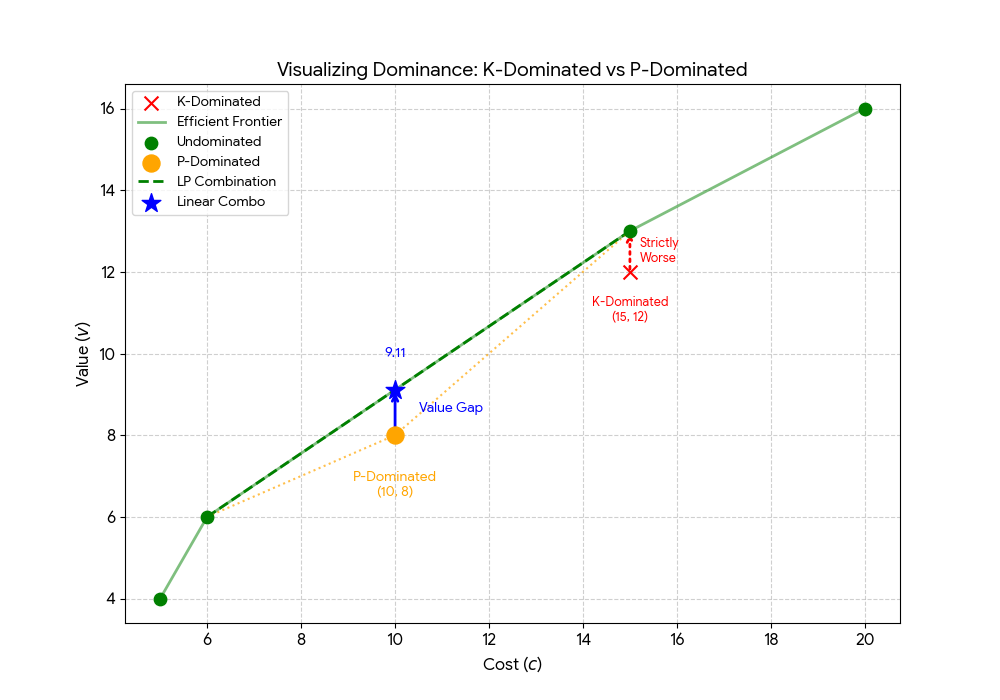
\includegraphics[width=5in]{figures/dominance_final_clean.png}
    \caption{类别1:k-dominated和类别2:p-dominated}
    \label{fig:my_label}
\end{figure}\par
将每个冒泡 $i$ 的决策过程视作从最低成本开始的增加补贴过程。\\
对于$j=1$，$\sum_i{c_{i1}}<B$否则问题P1、P2的可行域都是空集。
对于$j>1$当冒泡 $i$ 当前处于第 $j-1$ 档折扣，若将其增加补贴到第 $j$ 档折扣：
\begin{itemize}
    \item 边际成本增量：$\Delta c_{ij} = c_{ij} - c_{i(j-1)}\quad \forall i$
    \item 边际收益增量：$\Delta v_{ij} = v_{ij} - v_{i(j-1)}\quad \forall i$
\end{itemize}

定义该动作的\textbf{投资回报率(Return On Investment，ROI)}为：
\begin{equation}
\rho_{ij} = \frac{\Delta v_{ij}}{\Delta c_{ij}}\quad\forall i\quad \forall j
\end{equation}


%\textcolor{red}{命题2的intuition是什么？这个有什么作用（为什么放在这里）？是公认（通用）的吗？证明是你证的，还是已有文献给出的。给出文献}


\subsubsection{全局排序与贪心选择}
将所有冒泡的所有潜在加补动作(假设最初所有冒泡都给最小的补贴额$c_{i1},\forall i$,此时一定有$\sum_ic_{i1}<B$，记$c_{i(j'-1)}$ 到$c_{ij'}$为一次加补动作，$\forall j'>1$)放入一个全局集合，记为 $S_{all}$：
$$ S_{all} = \{ (i, j') \mid \forall i, \forall j'>1 \} $$\par
按照 $\rho_{ij}$ 从大到小对集合 $S_{all}$ 进行排序，得到有序序列：
$$ \text{Seq} = \{ \text{step}_1, \text{step}_2, \dots, \text{step}_N \} $$\par
其中 $\rho(\text{step}_k) \ge \rho(\text{step}_{k+1})$。

线性松弛问题 $P_2$ 的求解等价于：\textbf{按顺序执行这些升级动作，直到预算 $B$ 耗尽。}
设 $C_k$ 为执行前 $k$ 个动作的累计成本。由于预算有限，必然存在一个点$m$，使得：
\begin{equation}
C_{m-1} \le B < C_m
\end{equation}

\subsubsection{解的结构}
根据上述贪心过程，最优解 $\bm{z}^*$ 的取值被点 $m$ 划分为三类：

\begin{enumerate}
    \item \textbf{为1的部分} ($k < m$)：
    排序在点$m$之前的升级动作被执行。对于这些动作所属的冒泡，其决策变量最终停留在某个确定的高档位，即 $z_{ij} = 1$（整数）。

    \item \textbf{为0的部分} ($k > m$)：
    排序在点$m$之后的动作因预算不足被放弃。对应的高档位决策变量 $z_{ij} = 0$（整数）。

    \item \textbf{为分数的部分} ($k = m$)：
    这是唯一发生“预算耗尽”时刻的动作。为了花完剩余预算 $(B - C_{m-1})$，只能部分选取 $m$ 。
    该动作对应的冒泡 $i^*$ 是全局唯一取值为分数的样本。$m$对应的$v$也就是P1\eqref{eq:mckp}和P2\eqref{eq:smckp}的松弛间隙。
\end{enumerate}

\subsubsection{结论与近似误差}
综上所述，线性松弛解 $\bm{z}_c^*$ 在结构上仅包含一个分数项，其余均为整数。
令 $F_{\bm{z_c^*}}$ 为线性松弛最大收益，$F_{z^*}$ 为整数规划最大收益。由于仅有第 $m$ 个动作为分数，两者之差不会超过该动作带来的最大可能收益 $v_{max}$，因此两者之差的上界如下：
\begin{equation}
F_{\bm{z_c^*}} - F_{\bm{z^*}} < v_{\max}
\end{equation}\par
考虑到网约车场景下总收益 $F_{\bm{z^*}}$ 远大于单个收益 $v_{\max}$，因此该近似带来的相对误差趋近于0，如下所示:
\begin{align}
    \lim_{N\to \infty} F_{\bm{z^{*}}} - F_{\bm{z^*_c}} = 0
\end{align}

因此线性松弛解$\bm{z_c^*}$的整数部分可以视作原整数问题的最优解。
贪心算法将线性松弛问题的求解复杂度降低到了$\mathcal{O}\left(N\log \|J\| + N \log N +N \right) = \mathcal O (N\log N)$。
然而，当$N$极大时，求解速度仍较慢。因此，为进一步提升求解速度，可通过拉格朗日松弛，将该预算约束问题转化为无约束问题进行求解。



\subsection{拉格朗日对偶问题P3}

拉格朗日对偶将 NP-Hard 问题分解为易解的子问题。

\subsubsection{拉格朗日函数}

线性松弛问题 \eqref{eq:smckp} 的约束分为两类：
\begin{enumerate}
    \item 不等式约束（预算约束）：$\sum_{i}\sum_{j} z_{ij} \cdot c_{ij} - B \leq 0$
    \item 等式约束（每个个体选且仅选一个处理）：$\sum_{j} z_{ij} - 1 = 0, \forall i$
\end{enumerate}


附录证明了对于等式约束可以不松弛，解的效果是等价的。
因此在构造拉格朗日函数（Lagrangian Function）$L(\bm z,\lambda)$时只对不等式约束进行松弛，得到拉格朗日函数$L(\bm{z},\lambda)$：
\begin{align}
L(\bm{z}, \lambda) &= \sum_{i}\sum_{j} z_{ij} \cdot v_{ij} - \lambda \cdot \left( \sum_{i}\sum_{j} z_{ij} \cdot c_{ij}-B\right)\\
&= \sum_{i}\sum_{j} z_{ij} \cdot v_{ij} + \lambda B - \lambda \sum_{i}\sum_{j} z_{ij} \cdot c_{ij}  \\
&= \sum_{i}\sum_{j} z_{ij} \cdot (v_{ij} - \lambda \cdot c_{ij} ) + \lambda \cdot B 
\end{align}
\subsubsection{对偶函数}
对偶函数 $D(\lambda)$ 是关于$\lambda$的函数，
定义为：给定 $\lambda$ 时，$L(\bm{z}, \lambda)$ 关于 $\bm{z}$ 的最大值：

\begin{align}\label{eq:dualfunction}
D(\lambda) &= \max_{\bm{z}} L(z, \lambda) \\
&= \max_{\bm{z}} \left( \sum_{i}\sum_{j} z_{ij} \cdot (v_{ij} - \lambda \cdot c_{ij} ) + \lambda \cdot B  \right)\\
&= \lambda \cdot B + \underbrace{\max_{\bm{z_1}}  \sum_{j} z_{1j} \cdot (v_{1j} - \lambda \cdot c_{1j} ) + \cdots + \max_{\bm{z_N}}  \sum_{j} z_{Nj} \cdot (v_{Nj} - \lambda \cdot c_{Nj} )}_{\sum_{i}\max_{\bm{z_{i}}} \left(\sum_{j} z_{ij} \cdot (v_{ij} - \lambda \cdot c_{ij} ) \right)}\\
&=  \lambda \cdot B +\sum_{i}\max_{\bm{z_{i}}} \left(\sum_{j} z_{ij} \cdot (v_{ij} - \lambda \cdot c_{ij} ) \right) 
\end{align}

要使$L(\bm z,\lambda)$取最大值，需对每个个体 $i$ 选择能最大化 $(v_{ij} - \lambda c_{ij})$ 的处理 $j$：

令：
\begin{equation}
j^{*}(i, \lambda) = \arg\max_{j} (v_{ij} - \lambda \cdot c_{ij})
\end{equation}

\textbf{定义对偶函数解：}
对于给定的$\lambda$ 确定的决策变量  $\bm{z^d} = \{z_{ij}^d\}$ 为：
$$z_{ij}^d = 
\begin{cases} 
1 & \text{if } j = j^*(i,\lambda)\\ 
0 & \text{otherwise} 
\end{cases}$$
把$\bm {z^d}$代入$\eqref{eq:dualfuncation}$，可得：

\begin{equation}\label{eq:Dlambda}
\begin{aligned}
D(\lambda)&=\lambda \cdot B + \sum_i(v_{ij^*(i,\lambda)}-\lambda \cdot c_{ij^*(i,\lambda)})\\
&= \lambda \cdot \left( B-\sum_{i} c_{ij^*(i,\lambda)} \right) + \sum_{i} v_{ij^*(i,\lambda)}
\end{aligned}
\end{equation}

\subsubsection{对偶问题}
基于对偶函数$D(\lambda)$ \eqref{eq:Dlambda}，其对应的对偶问题如下所示：
\begin{equation}\label{eq:dual_problem}
\min_{\lambda \ge 0} D(\lambda)
=\min_{\lambda \ge0}\left(\lambda \cdot \left(B-\sum_ic_{ij^*(i,\lambda)}\right)+\sum_iv_{ij^*(i,\lambda)}\right)
\end{equation}

该问题的最优解可通过求导得到。然而，由于\eqref{eq:dual_problem}中$j^*(i,\lambda)$为分段线性函数，所以对偶函数$D(\lambda)$存在不可导的点。

常用的替代方案为用次梯度进行求导计算\citep{boyd2004convex}。$D(\lambda)$的次梯度如下所示：
\begin{align}
D'(\lambda) &= \frac{\partial D(\lambda)}{\partial \lambda} \\
&=  B-\sum_{i} c_{ij^*(i,\lambda)}
\end{align}
$\lambda^*$可在$D'(\lambda)=0$时求得。

为求解 $D'(\lambda) \approx 0$，常见两种数值方法，分别为（1）梯度下降法以及（2）二分法。下文对两种方法进行介绍。

\paragraph{方法一：梯度下降法 (Gradient Descent)}
此方法利用梯度方向逐步更新 $\lambda$，直到总成本逼近预算 $B$（因目标是最小化，改用梯度下降）。
\begin{algorithm}[H]
\caption{梯度下降求解 $\lambda^*$}
\begin{algorithmic}[1]
\State 初始化：$\lambda=0$，学习率$\alpha$，误差阈值$\epsilon$，目标$B$
\State 计算 $j^*_i = \underset{j}{\operatorname{argmax}} (v_{ij} - \lambda c_{ij}), \forall i$，并求 $C_{\text{total}} = \sum_i c_{ij^*_i}$
\While{$|B - C_{\text{total}}| \ge \epsilon$}
    \State $\lambda = \lambda - \alpha \cdot (C_{\text{total}} - B)$ 
    \State 更新 $j^*_i$ 和 $C_{\text{total}}$（同步骤2）
\EndWhile
\State \Return $\lambda^* = \lambda$
\end{algorithmic}
\end{algorithm}

\paragraph{方法二：二分法 (Bisection Method)}
由于 $h'(\lambda)$ 关于 $\lambda$ 单调递减（$\lambda$ 越大，选的补贴方案成本越低，总成本越低），使用二分法快速逼近零点。

\begin{algorithm}[H]
\caption{二分法求解 $\lambda^*$}
\begin{algorithmic}[1]
\State 初始化：$\lambda_{\text{left}}=0$, $\lambda_{\text{right}}= \max\limits_{i,j}\frac{v_{ij}}{c_{ij}}$, $\epsilon$ (误差阈值)，目标预算$B$
\While{$\lambda_{\text{right}} - \lambda_{\text{left}} \ge \epsilon$}
    \State $\lambda_{\text{mid}} = (\lambda_{\text{right}} + \lambda_{\text{left}})/2$
    \State 计算 $j^*(i,\lambda) = \underset{j}{\operatorname{argmax}} \left( v_{ij} - \lambda_{\text{mid}} c_{ij} \right), \forall i$
    \State $C_{\text{total}} = \sum_i c_{ij^*(i,\lambda)}$
    \State $h'(\lambda_{\text{mid}}) =  B - C_{\text{total}} $
    \If{$h'(\lambda_{\text{mid}}) \ge 0$}
        \State $\lambda_{\text{right}} = \lambda_{\text{mid}}$ \Comment{预算剩余，需减小$\lambda$}
    \Else
        \State $\lambda_{\text{left}} = \lambda_{\text{mid}}$ \Comment{成本超支，需增大$\lambda$} 
    \EndIf
\EndWhile
\State \Return $\lambda^* = (\lambda_{\text{left}} + \lambda_{\text{right}})/2$
\end{algorithmic}
\end{algorithm}
\subsubsection{对偶问题最优解}
在通过上述方法解出来最优的$\lambda^*$后，对应的决策变量$\bm z^{d}(\lambda^*)$:
\begin{align}
z_{ij}^{d*} = 
\begin{cases}
1, & \text{if } j = \arg\max\limits_{j} \left( v_{ij} - \lambda^* \cdot c_{ij} \right) \\ 
0, & \text{otherwise} 
\end{cases}
\end{align}

Slater条件：对于一个凸问题，若不等式约束为仿射约束，只要可行域非空，那么该凸问题和它的对偶问题一定是强对偶,即
\begin{align}
F(\bm z^d(\lambda^*)) = F(\bm z_c^{*})
\end{align}

该线性松弛问题满足Slater条件，具有强对偶性：
\begin{align}
F(\bm z^d(\lambda^*)) = F(\bm z_c^{*}) 
\end{align}

由\eqref{eq10}可知整数规划问题和线性松弛问题的松弛间隙有界

\begin{align} 
F(\bm z^*)\leq F(\bm z_c^*)\leq F(\bm z^*) + \max_{i,j} v_{ij}
\end{align}
因此对偶求解的结果和整数规划问题的近似比为\par
$$1\leq \frac{F(\bm z^d(\lambda^*))}{F(\bm z^*)}\leq 1+\max_{ij}\frac{v_{ij}}{F(z^*)}$$

\section{在线问题P4}
从运筹的角度来看，将补贴发放建模为一个多选择的背包问题，存在一个假设：决策时可以对所有冒泡做决策,即决策向量$Z$为$N\cdot M$维。\par
但是实际上冒泡是逐个到达，且必须对到达对冒泡立刻决策
，因此本质上这是一个在线多选择的背包问题，即
考虑冒泡到达序列为$\sigma$
$$\sigma = \{(v_1, c_1), (v_2, c_2), \dots, (v_n, c_n), \dots\}$$\par
第$t$个冒泡到达时,决策变量$z_{tj} \quad\forall j$必须给定，且仅依赖于第$t$个冒泡及以前的信息。用关系$H$表示这一限制,则$z_{tj}=H((v_{1j}, c_{1j}), \dots, (v_{tj}, c_{tj}); z_1, \dots, z_{{t-1}j})$
\begin{equation} \label{eq:omckp}
\begin{aligned}
\max_{\bm z} \quad &  \sum_{i}\sum_{j}v_{ij}z_{ij} \\
\text{s.t.} 
\quad 
& \sum_{i}\sum_{j} c_{ij} z_{ij} \le B  \\
& \sum_{j} z_{ij} = 1, \quad \forall i \\
&z_{tj} = H((v_{1j}, c_{1j}), \dots, (v_{tj}, c_{tj}); z_1, \dots, z_{{t-1}j})\\
& z_{ij} \in \{0, 1\}
\end{aligned}
\end{equation}\par
在线背包的求解主要的求解方法：
\begin{itemize}
    \item 基于阈值：文献\cite{chakrabarty2008online}
定义了一个基于背包当前填充比例 $r$ 的阈值函数 $\Psi(r)$。该函数用于衡量冒泡单位收益成本之比（即 $v/c$）是否足够高，以决定是否接纳该物品。\par
$$\Psi(r_i) = \left( \frac{Ue}{L} \right)^{r_i} \left( \frac{L}{e} \right)$$
\begin{itemize}
    \item $r_i$：$\frac{\sum_{(i-1)}\sum_j c_{(i-1)j}z_{(i-1)j}}{B} \forall i>1$
    \item L：$\frac{v_{ij}}{c_{ij}} \quad\forall i\quad\forall j$的上界
    \item U：$\frac{v_{ij}}{c_{ij}}\quad\forall i\quad\forall j$的下界
    \item $e$：自然对数
\end{itemize}
\par
对于第$i$个冒泡，在满足$\frac{v_{ij}}{c_{ij}}>\Psi$的所有$j$中选取$\max_j{v_{ij}}$的$j^*$,对于冒泡$i$,仅有$z_{ij^*}=1$。上述在线问题求解的最优决策结果设为$F(\bm{z_o^*})$,离线算法（从一开始就得到了全部输入）的最优决策结果为$F(\bm{z^*})$。
\begin{equation}
\begin{aligned}
F(\bm{z^*})-F(\bm{z_o^*})\le (\ln(U/L)+1)\cdot F(\bm{z_o^*})
\end{aligned}
\end{equation}
    \item 在线对偶\cite{buchbinder2009online}
    \item 多臂赌博机：文献\cite{badanidiyuru2018bandits}(还没看懂)
\end{itemize}
\section{didi业务}
\subsection{数据类型}

1. 观测数据 (Observational Data)

在观测数据中，决策变量 $z$ 或策略选择 $t$ 是由历史上的既定策略函数 $h(\cdot)$ 决定的。

生成机制： 策略分配 $t$ 与请求特征 $\mathbf{x}_i$ 之间存在相关性。即存在一个函数 $h: \mathcal{X} \rightarrow \mathcal{T}$，使得 $t_i = h(\mathbf{x}_i)$。

混杂因素 (Confounding)： 由于决策是基于特征 $\mathbf{x}_i$ 做出的，而特征 $\mathbf{x}_i$ 同时也会影响最终结果 $y_i$（如高消费用户本身完单概率就高），因此特征 $\mathbf{x}_i$ 成为了混杂变量。

预测模型应用： 预估值 $\hat{y}_{ij} = P(y = 1 \mid \mathbf{x}_i, t = j)$ 在观测数据下反映的是在特定历史偏置下的条件概率。直接使用此数据进行因果推断会产生偏差，因为 $\mathbf{x}_i$ 决定了用户进入不同策略组的概率。

2. 随机分配数据 (Randomized Data / RCT)

在随机分配（如 A/B 测试）中，策略选择 $j$ 与请求特征 $\mathbf{x}_i$ 是相互独立的。

生成机制： 决策变量 $z_{ij}$ 的取值不依赖于 $\mathbf{x}_i$，而是通过随机过程产生。这意味着：$$P(t = j \mid \mathbf{x}_i) = P(t = j)$$

因果推断： 在这种数据下，表中所述的 Uplift $\tau(\mathbf{x}_i)$（增益）可以被更准确地估计。由于消除了特征对分配的影响，不同策略组（Treatment vs Control）之间的结果差异可以被直接归因于策略 $j$ 本身，而非用户画像的差异。

评价指标：  Qini 系数 $Q(\pi)$ 通常用于评估在随机实验数据或具有真值的验证集上，策略 $\pi$ 对不同人群的排序能力，即能否优先识别出那些“不给补贴不转化，给了补贴才转化”的用户。


\subsection{乘客定价业务逻辑}
乘客定价团队属于mpt下供需调节策略部门。通过调整乘客（C端）、司机（B端）的价格，来调节市场的供需，进而影响平台的成交量、收入和毛利。乘客定价主要是负责计算动态调价以及智能呼返补贴的部分。（除了乘客定价部门负责的定价业务还有其他部门负责的勾选、推荐、广告流量、城市补贴预算等业务）。

\begin{figure}[!h]
    \centering
    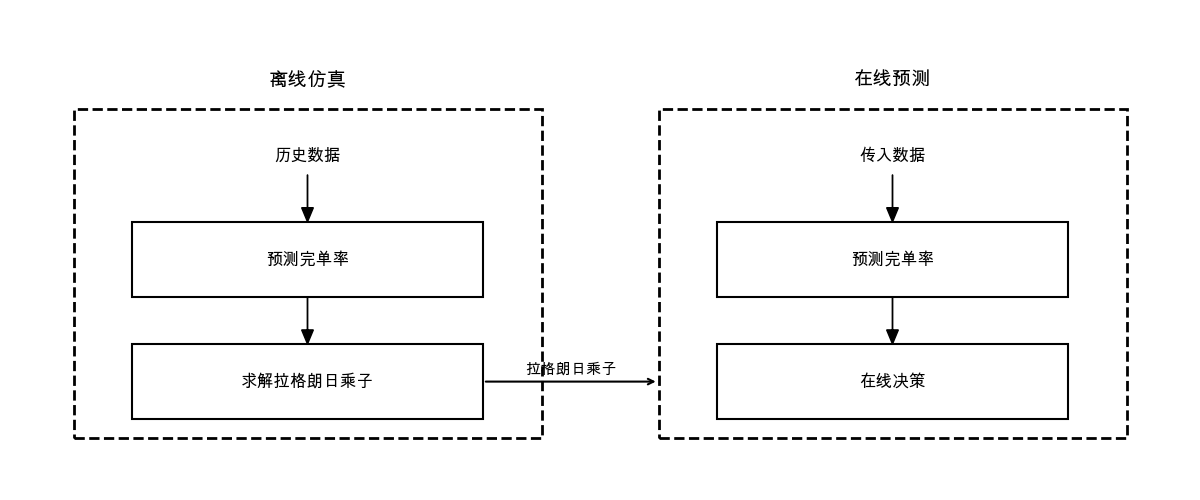
\includegraphics[width=5in]{figures/流程示意图.png}
    \caption{整体示意图}
    \label{fig:my_label}
\end{figure}
\textbf{业务名词}

\begin{enumerate}
\item 冒泡：用户输入起终点
\item 出价：系统给出每个品类的定价和折扣
\item 发单：用户选择发单（选某一品类或同时选多个品类）或不发单
\item 应答：系统派单-司机应答
\item 完单：乘客向平台支付车费，平台向司机支付司机费
\item 预测：模型根据特征预估冒泡完单率
\item 仿真：离线产出最优$\lambda$
\item 打分公式：线上决策的依据，由预测模型预估值和离线产出的$\lambda$两部分组成
\end{enumerate}
\textbf{主要定价品类}\\
不同品类完单占比：
\begin{equation}
  \text{快车} : \text{特惠} : \text{惊喜} : \text{其他品类} \approx 2 : 4 : 1 : 2
\end{equation}
\text{快车一口价}
\begin{itemize}
    \item $T$：\{104, 103, 100, 97, 95\}；
    \item 预测值：预测每种折扣下的应答概率；
    \item 约束：快车相比不发折扣（全为100折）完单不降，快车毛利不降；
    \item 目标：最大化业务收益
\end{itemize}
\text{特惠呼反}
\begin{itemize}
    \item $T$：\{90, 85, 80, 75, 70\}；
    \item 预测值：预测每种折扣下的应答概率；
    \item 约束：特惠相较于快车降低的价格作为补贴，补贴总量要在一定预算范围；
    \item 目标：最大化业务收益
\end{itemize}
此外除了快车和特惠还有专车、出租车等品类。

\subsubsection{基础预估价}司乘两端预估价(快车、特惠)都是依赖地图侧提供预估时长和预估里程计算获得:\par
乘客基础预估价：$P^{base}_i=a\cdot S_i+b\cdot T_i$\par
司机基础预估价：$P^{driver}_i$\par
注：此处不考虑司机端的定价策略
\subsubsection{快车一口价}
快车一口价会在基础预估价的基础上“二次改价”：\par
$P^{kc}_i=P^{base}_{ij}\cdot t_{ij}$\par
折扣（treatment、决策、动作）为$t_{ij}\in\{95,97,100,103,104\} \forall i$，
\par$P^{kc}_i$会作为泛快品类（快车、特惠、惊喜）的交易额的计算口径（GMV）。\par
快车一口价对应的运筹问题：
\begin{equation} 
\begin{aligned}
\max_{\bm{z}}\quad & \sum_{i }\sum_{j} v_{ij} z_{ij} \\
\text{s.t.} \quad & \sum_{i }\sum_{j } w_{ij} z_{ij} \geq 0 &  \text{快车毛利约束}\\
& \sum_{i}\sum_{j} c_{ij} z_{ij} \geq 0 &\text{快车完单约束} \\
& \sum_{j \in J} z_{ij} = 1, \quad \forall i \in I  \\
& z_{ij} \in \{0,1\}, \quad \forall i \in I, j \in J \\
v_{ij} &= P^{base}_i \cdot t_{ij} \cdot \widehat{ABR^{kt}_{ij}} \\
w_{ij} &= (P^{base}_i \cdot t_{ij} - P^{driver}_i) \cdot \widehat{ABR^{kc}_{ij}} \\
&\quad - (P^{base}_i \cdot t_{i,100} - P^{driver}_i) \cdot \widehat{ABR^{kc}_{i,100}} \\
c_{ij} &=  \widehat{ABR^{kc}_{ij}}-\widehat{ABR^{kc}_{i,100}} \\
\end{aligned}
\end{equation} 
\begin{itemize}
    
    \item $i$：表示每一条定价样本，即冒泡
    \item $j \in J$：表示所有 treatment 的集合
    \item $\widehat{ABR^{kt}_{ij}}$：表示某一个冒泡在treatment $j$下快车和特惠应答率之和的预估值
    \item $\widehat{ABR^{kc}_{ij}}$：表示某一个冒泡在treatment $j$下快车应答率的预估值
    \item $DriverFee_i$:司机费用
    \item $Discount_{j}$：表示某在treatment $j$下对应的折扣
    \item $z_{ij}$：表示第 $i$ 个冒泡是否选择 treatment $j$
    \item $\widehat{ABR^{kc}_{i,100}}$：表示一个冒泡在100折下快车应答率的预估值
\end{itemize}
和上述证明对应，
打分公式：$$\begin{aligned}
score_{ij} = v_{ij}+\lambda_1\cdot w_{ij}+\lambda_2\cdot  c_{ij}
\end{aligned}
$$\\
证明见附录二。

对于线上每个冒泡，预测模型会预估冒泡在折扣$t_{ij}$（95，97，100，103，104）下的快车应答率和快特（快车加特惠）的应答率，并结合离线仿真得到的$\lambda_1$、$\lambda_2$，计算不同折扣下的score。socre最大的treatment为实际出价折扣。
\subsubsection{特惠呼反}
特惠快车是在快车一口价的基础上发放折扣，上游资源分配会给定分城市分时段的目标补贴率，补贴率SR定义为$(P_{kc}-P_{th})/P_{kc}$也就意味着$P_{th}=P_{kc}*(1-SR)$
特惠呼反对应的运筹问题：
\begin{equation} 
\begin{aligned}
\max  & \sum_{k \in K}\sum_{i \in I}\sum_{j \in J} P_{ijk} \cdot \widehat{ABR_{ijk}} \cdot z_{ijk} \\
{\rm s.t.} & \sum_{i \in I}\sum_{j \in J} (P_{base,i} \cdot discount_{j}\cdot\hat{ABR_{th,ij}} /P_{base,i} )\cdot z_{th,ij} \leq SR  \\
& \sum_{j \in J} z_{ijk}  = 1, \  \forall i \in I \forall k \in K  &\\
& z_{ijk} \in \{0,1\}  
\end{aligned}
\end{equation} 



\subsection{乘客定价的两大组成部分}
在滴滴的场景中，决策$T$为业务折扣，输入特征$X$是冒泡的ODT（时间地理以及供需特征）预测值$Y$为应答概率（abr）。\par
但在定价场景中，我们需要回答的问题是：“对于特征$X$，如果改变价格 $T$，完单率 $Y$ 会如何变化？”，从而实现学习到什么特征的人群对价格不敏感，什么样的人群对价格十分敏感。用函数$f$表示$X$、$T$、$Y$之间对关系
$$Y = f(X, T)$$\par
因为我们需要准确估计 $f(X, T)$ 中的 $T$ 的贡献，从而在线上时特征$X$到达，我们选出最优的$t^*$。但是在观察数据中，$X$ 和 $T$ 相关，模型无法区分 $Y$ 的变化是由 $X$ 引起的，还是由 $T$ 引起的。\par
RCT数据通过随机发放折扣，让 $X$ 和 $T$ 不相关（正交）。$X$ 部分负责解释用户的基础属性。$T$ 部分负责解释价格带来的额外增量。

\begin{enumerate}
    \item 观测数据：T由当前线上的模型$m(X)$+$\lambda$决定,和X不独立，因此不同折扣的数据特征分布不一致。
    \item 随机分配数据：T随机发放，和X独立，因此不同折扣的数据特征分布一致。
\end{enumerate}
\subsubsection{prediction}




\begin{enumerate}
    \item $v_{ij}=V({abr}_{ijk})$
    \item $c_{ij}=C({abr}_{ijk})$
\end{enumerate}
以快车一口价场景为例：\par
$V_{ij}=\sum_{k \in K}\sum_{i \in I}\sum_{j \in J} P_{ijk} \cdot \hat{ABR_{ijk}} \cdot z_{ijk}$\par
$C_{1ij}=(P^{base}_i \cdot Discount_{ij}-DriverFee_i) \cdot ABR_{kc,ij} -  (P^{base}_i \cdot Discount_{i,100} - DriverFee_i) \cdot ABR_{kc,i,100}$对应问题（22）中的约束一\par
$C_{2ij}=\Delta ABR_{kc,ij}$ 对应问题（22）中的约束二



\paragraph{input}
随机分配数据
\begin{enumerate}
    \item ODT特征 $X_{i}$例如供需、城市、天气、表单
    \item 应答标签 $Y_{ij}$在快车一口价中，应答标签为5种快车一口价[95,97,100,103,104]下该冒泡是否以快车、特惠应答。例如[0,0,0,1,0][0,0,0,0,0]表示为快车103折应答
    \item 补贴决策 $Z_{ij}$
    [0,0,0,1,0]表示该用户看到的快车一口价为103折

\end{enumerate}


\paragraph{model}
\begin{enumerate}
    \item 因果树模型

    \item 深度模型     
    \begin{enumerate}
        \item $\ell_{\text {BCE}}(\hat y,y)= -[y \cdot \log(\hat y) + (1-y)\cdot \log(1-\hat y)]$ (计算预测完单率$\hat{y}$和实际完单$y$的二元交叉熵损失。
        \item parirwiseloss =first\_pairwise\_loss = torch.log(
                1 + torch.exp(mask * (y\_treatment-y\_control)
                （保证预测的完单率满足：价格越低，完单率越高）
    \end{enumerate}
\end{enumerate}


\paragraph{output}
应答概率
$\hat{{abr}}_{ijk}$:冒泡i在给出折扣j下品类k的应答率\par
$\hat{Y_{ijk}}=f_\theta(X_i)$\par
Y(kc):[0.2,0.15,0.10,0.05,0.03]\par
Y(kt):[0.4,0.38,0.36,0.34,0.32]

\subsubsection{simulation}


1. 问题背景：

在现有文献（\cite{chen2023two}, \cite{zhang2021bcorle}, \cite{zhou2024decision}）中，补贴分配通常被建模为预算 $B$ 约束下的优化问题。理论上，拉格朗日乘子 $\lambda$ 与预算 $B$ 存在严格的单调对应关系（一一对应），求解通常采用二分法来寻找使得预算约束紧致（即预算刚好耗尽）的最优 $\lambda^*$。

2. 实际场景：

然而，在实际业务场景（如滴滴的补贴发放）中，固定的预算金额 $B$ 往往是未知的或动态变化的。实际控制变量通常是期望补贴率（Subsidy Rate,SR）。与预算约束不同，当约束条件转换为期望补贴率时，$\lambda$ 与补贴率之间不再保持一一对应的单调关系，即同一个补贴率可能对应多个 $\lambda$ 值。在此情形下，运筹优化问题的目标转变为：在满足给定补贴率约束的所有候选 $\lambda$ 中，寻找使得总交易额（GMV）最大化的那个 $\lambda$。

3. 求解策略：

为了解决上述问题，滴滴仿真并没采用基于固定预算 $B$ 的二分查找法，改为采用对 $\lambda$ 空间进行遍历的策略。算法逻辑为直接遍历 $\lambda$ 的取值范围，计算每个 $\lambda$ 对应的交易总额和补贴金额，进而推导出对应的补贴率。最后，在符合目标补贴率的解集中，选取对应 GMV 最大的 $\lambda$。并且在遍历过程中，为了兼顾计算效率与精度，采用非均匀采样。即在 $\lambda$ 较小的区域进行高密度采样（密取），在 $\lambda$ 较大的区域进行稀疏采样（疏取）。

4. 算法分析：

该方法的优势主要体现在以下两点：合理性：相比于并不确定的金额约束，约束补贴率更符合业务实际逻辑。仿真模型能够处理非单调的映射关系，确保在多解情况下选出全局最优的 GMV。计算效率：避免冗余计算：传统的二分法仅针对单一预算 $B$ 求解，若需评估不同预算或补贴率下的情况，需重复多次二分查找，计算成本高且中间结果被浪费。全景映射：通过遍历 $\lambda$，我们一次性构建了“$\lambda$ - 补贴率 - GMV”的完整映射关系表。这不仅避免了针对特定 $B$ 的重复计算，还支持在不同约束条件下快速查询最优策略，极大提升了求解效率。

仿真是滴滴离线求解$\lambda^*$的过程：

\begin{enumerate}
    \item 取一批近期的观测数据（一般为一周）的特征$X$
    \item 将观测数据输入到构建的预测模型$m(X)$,模型输出是不同折扣下的应答率$\widehat{abr_{pre}} $
    \item 遍历$\lambda$组合，结合预测模型$m(X)$的输出组成一个打分公式，得到$\hat T$
    \item 把$(X,\hat T)$输入到仿真模型$m_{sim}(X,\hat T)$，仿真模型根据特征预估每个数据在$\hat T$折扣下的完单率$\widehat{cbr_{sim}}$。
    \item 将每个个体的完单率和对应的折扣、订单金额相乘，将所有个体聚合得到关于$\lambda$对应的总订单额$G(m(X),\lambda)$,以及补贴金额$B(m(X),\lambda)$。
    \item 补贴率$SR(m(x),\lambda)=\frac{G(m(X),\lambda)}{B(m(X),\lambda)}$。对于相同的SR取值：按照$G$排序，使得$G^*(m(X),\lambda^*)$最大的$\lambda^*$就是补贴率$SR(m(x),\lambda)$下对应的最优$\lambda$
    \item 得到补贴率与$\lambda^*$对应的字典。
\end{enumerate}

\begin{figure}[!h]
    \centering
    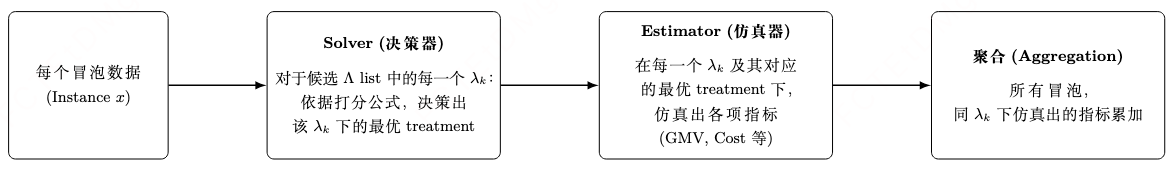
\includegraphics[width=0.95\linewidth]{figures/仿真简化流程图.png}
    \caption{仿真简化流程图}
    \label{fig:my_label}
\end{figure}





\begin{itemize}
    \item $x \in \mathcal{X}$: 单个冒泡数据。
    \item $M(x)$：预测模型
    \item $M_{sim}(x)$：仿真模型
    \item $\widehat{abr_{pre}}$：预测模型的预估值(应答率)
    \item $\widehat{cbr_{sim}}$：仿真模型的预估值(完单率)
    \item $\mathcal{T}$: 折扣（Treatments）。
    \item $\Lambda = \{\lambda_1, \lambda_2, \dots, \lambda_k\}$: 遍历的拉格朗日乘子。
    \item $\mathbf{O}$ : 业务指标（如 \text{GMV}, \text{C}）。
\end{itemize}

\begin{figure}
    \centering
    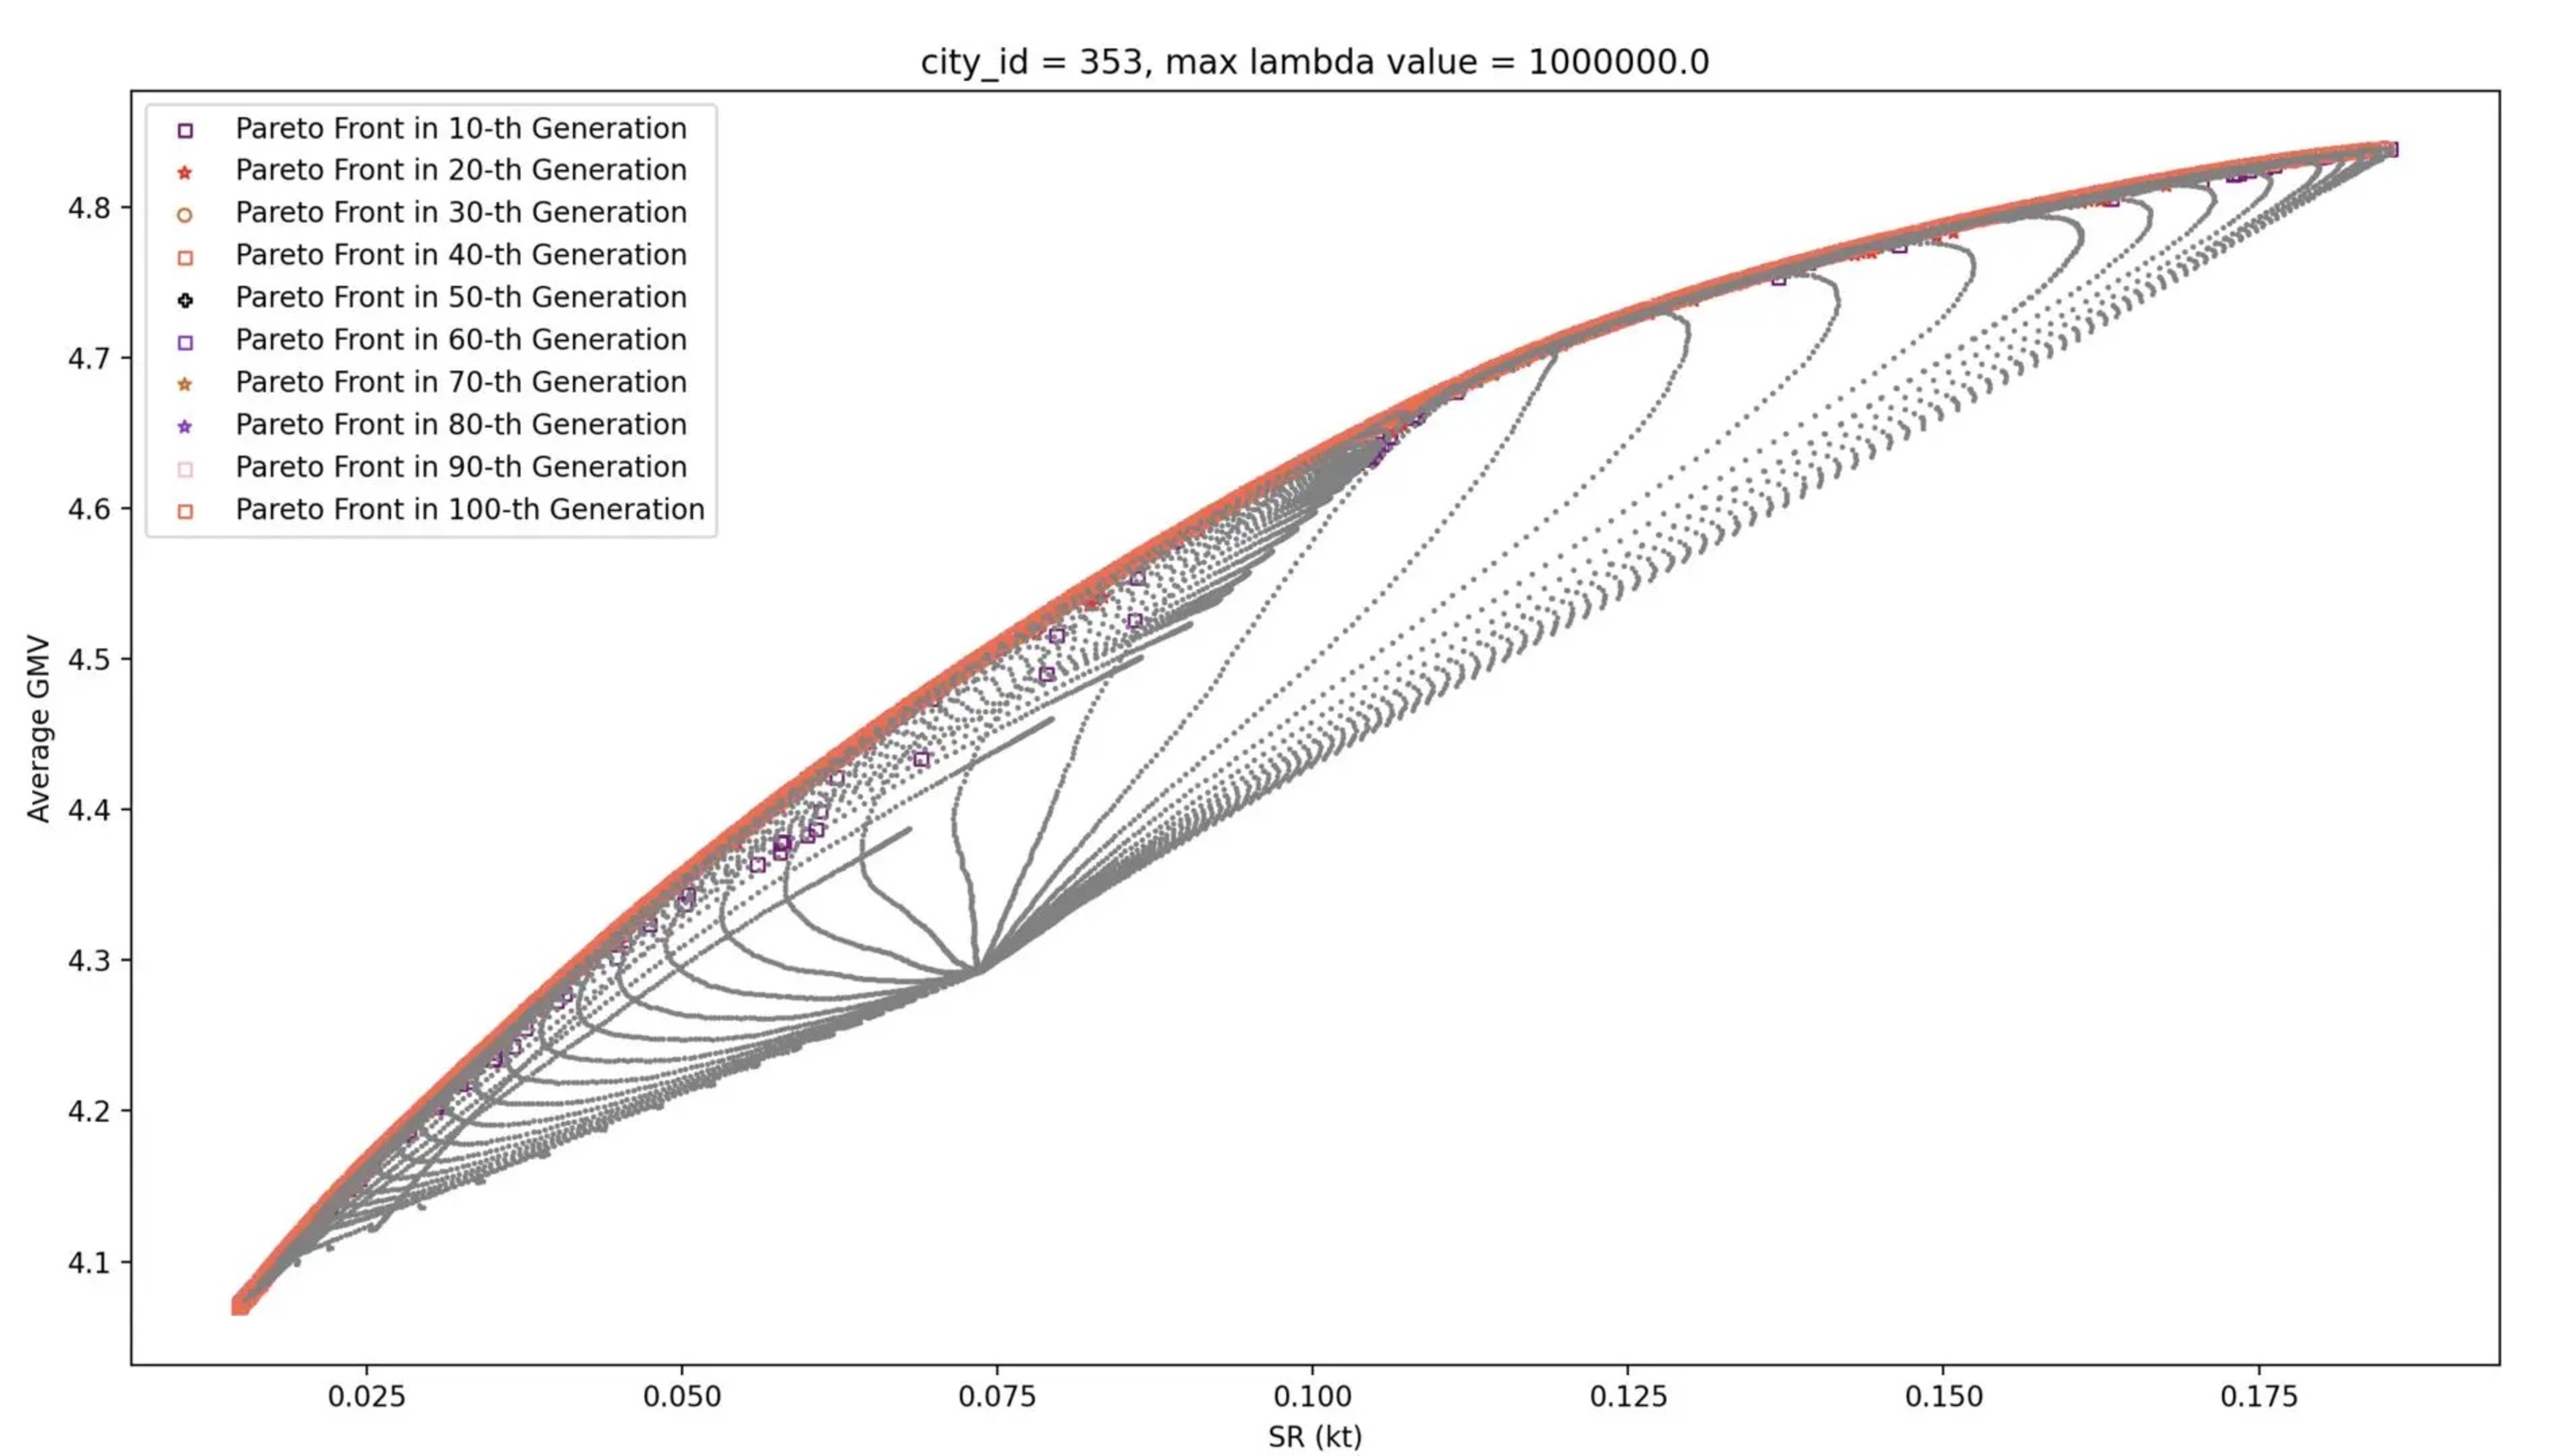
\includegraphics[width=\linewidth]{figures/sr-gmv-simulation.pdf}
    \caption{仿真结果}
    \label{fig:placeholder}
\end{figure}


\subsection{评估方法}
线上出价流程用数学表达为一个从特征空间 $\mathcal{X}$ 到干预空间 $\mathcal{T}$ 的映射函数（即预测模型+拉格朗日乘子） $h: \mathcal{X} \rightarrow \mathcal{T}$。在进行在线 A/B 实验前，我们需要在离线测试集上评估该映射函数 $h$ 的预期表现。

由于训练数据中每个样本 $(x^{(i)}, t^{(i)}, y^{(i)})$ 仅包含在一个特定动作 $t^{(i)}$ 下的反馈 $y^{(i)}$（即标签仅部分观测），我们无法直接计算模型在所有可能动作下的损失函数。因此，离线评估指标分为两类：
\begin{itemize}
    \item 排序指标：AUUC 和 Qini。主要评估预测模型的输出。
    \item 结果指标：期望输出矩阵（EOM）和仿真业务指标。主要利用统计估计方法，计算策略 $h$ 在测试集上的期望收益 $\mathbb{E}[Y]$。
\end{itemize}

\subsubsection{期望输出矩阵 (\cite{zhao2017uplift})}

\begin{figure}[!h]
    \centering
    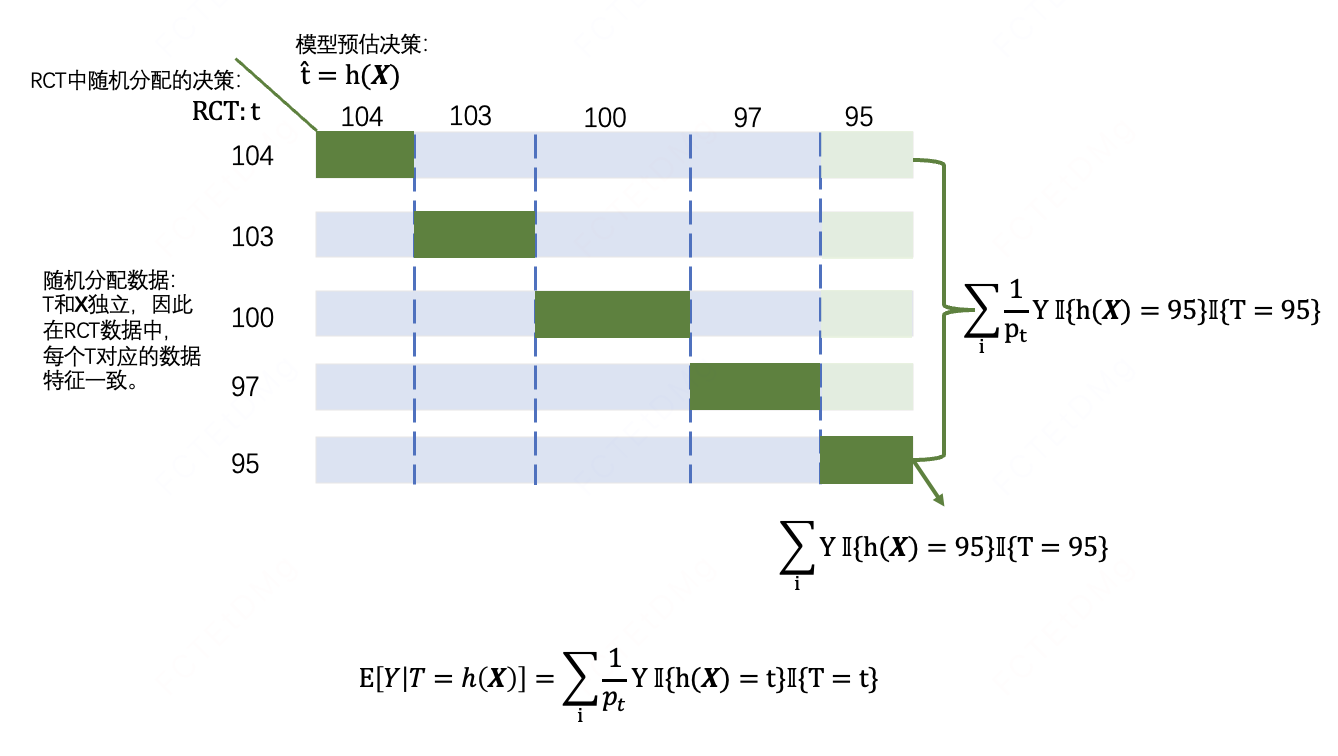
\includegraphics[width=5in]{figures/EOM.png}
    \caption{EOM期望输出矩阵计算示意图}
    \label{fig:my_label}
\end{figure}
\begin{equation}
    r_i = \begin{cases} 
    \frac{y_i}{p_{t_i}} & \text{if } h(\bm{x}_i) = t_i \\
    0 & \text{if } h(\bm{x}_i) \neq t_i
    \end{cases}
\end{equation}
期望收益：
\begin{equation}
    E[Y|T=h(\mathcal{X})]= \frac{1}{N}\sum_{i} r_i 
\end{equation}

该指标将评估问题转化为一个加权平均问题，直接量化模型 $h$ 的预期结果。

\subsubsection{仿真业务指标}
对于一批观测数据通过预测模型$m(X)$预估完单率后遍历$\lambda$，计算出对应的$\hat T(\lambda)$,并将$X$和$\hat T$输入到仿真模型$m_{sim}(X,\hat T)$仿真出相关的业务指标$G(m(X),\lambda)$，从而实现对策略的评估。\par

虽然仿真和EOM对模型$m(X)+\lambda$的评估方式不同，但是都是对最终策略的一种评价指标。理论上应该具有一致性：
\paragraph{仿真和EOM一致性理论证明}
在RCT数据分布无偏的条件下，论文\cite{zhao2017uplift}证明了 EOM 是策略真实收益的无偏估计，即：
\begin{equation}
    \mathbb{E}[\text{EOM}(h)] = E[Y|T=h(\mathcal{X})]
\end{equation}
设仿真模型 $m_{sim}$ 在特征 $\bm{X}$ 和折扣 $T$ 下的预测误差为 $\epsilon(\bm{x}, t)$，定义为仿真值与真实条件期望之差：
\begin{equation}
    \epsilon(\bm{x}, t) = m_{sim}(\bm{x}, t) - \mathbb{E}[Y \mid \mathcal{X}=\bm{x}, T=t]
\end{equation}
假设仿真模型在当前数据分布下的预测误差绝对值是有界的，即存在常数 $\delta \geq 0$，使得对于任意样本 $(\bm{x}, t)$ 满足：
\begin{equation}
    |\epsilon(\bm{x}, t)| \leq \delta
\end{equation}
对于策略 $h$，仿真评估指标 $J_{sim}(h)$ 与 EOM 期望指标 $J_{eom}(h)$ 的差距 $\Delta(h)$ 可以推导如下：
\begin{equation}
\begin{aligned}
    \Delta(h) &= \left| J_{sim}(h) - \mathbb{E}[\text{EOM}(h)] \right| \\
    &= \left| \mathbb{E}_{\mathcal{X}}[m_{sim}(\mathcal{X}, h(\mathcal{X}))] - \mathbb{E}_{\mathcal{X}}[\mathbb{E}[Y \mid \mathcal{X}, T=h(\mathcal{X})]] \right| \\
    &= \left| \mathbb{E}_{\mathcal{X}} \left[ m_{sim}(\mathcal{X}, h(\mathcal{X})) - \mathbb{E}[Y \mid \mathcal{X}, T=h(\mathcal{X})] \right] \right| \\
    &= \left| \mathbb{E}_{\mathcal{X}} [\epsilon(\mathcal{X}, h(\mathcal{X}))] \right|
\end{aligned}
\end{equation}
根据绝对值的性质 $|\mathbb{E}[Z]| \leq \mathbb{E}[|Z|]$，我们可以进一步得到误差的上界：
\begin{equation}
    \Delta(h) \leq \mathbb{E}_{\mathcal{X}} [ |\epsilon(\mathcal{X}, h(\mathcal{X}))| ] \leq \delta
\end{equation}
\textbf{证明结论}：
仿真评估与 EOM 评估之间的差距 $\Delta(h)$ 严格受限于仿真模型的逐点预测误差界 $\delta$。只要仿真模型的最大误差 $\delta$ 在可接受范围内，仿真评估结果就能作为 EOM 指标（即真实策略收益）的有效代理，两者具备理论上的一致性边界。
\paragraph{仿真与EOM一致性实验分析}

快车一口价业务的深度模型$m(X)$和拉格朗日乘子对：$\lambda_1,\lambda_2$。
实验了在仿真中表现前三的拉格朗日乘子:$$\bm{\lambda}_1,\bm{\lambda}_2,\bm{\lambda}_3$$探究其在EOM上的表现。
对于一组模型$m(X)$和$\bm \lambda$
\begin{itemize}
    \item 仿真模型：OBS数据，$\hat Y=m_{sim}(X,T)$
    \item EOM：RCT数据，$Y= \mathbb{E}[Y|T=h(X)]$
\end{itemize}
\begin{table}[htbp]
\centering
\caption{仿真指标与 EOM 指标对比}
\label{tab:comparison}
\resizebox{\textwidth}{!}{%
\begin{tabular}{|c|c|c|c|c|c|c|c|}
\hline
\multirow{2}{*}{序号} & \multicolumn{2}{c|}{参数设置} & \multicolumn{4}{c|}{仿真指标} & \multicolumn{1}{c|}{EOM指标} \\ \cline{2-8} 
 & lambda1 & lambda2 & kt\_gmv\_uplift & kc\_gmv\_up & kc\_pr\_uplift & kc\_abr\_uplift & kt\_gmv\_uplift \\ \hline
1 & 7.7469 & 35.9461 & 0.01 & 0.0249 & 0.0114 & 0.0527 & 0.02554 \\ \hline
2 & 59.9551 & 168.106 & 0.0046 & 0.026 & 0.0262 & 0.0373 & 0.02043 \\ \hline
3 & 101 & 279.7984 & 0.003 & 0.0282 & 0.0227 & 0.0397 & 0.01756 \\ \hline
\end{tabular}%
}
\end{table}
\subsubsection{AUUC}
AUUC (Area Under the Uplift Curve) 类似于分类任务中的 AUC 指标。不关注预测值的绝对误差（MSE），而是关注模型对样本的相对排序质量。计算的是在不同覆盖率 $\alpha$ 下，累积增益曲线（Lift Curve）下的面积。AUUC 越高，说明模型越擅长将高响应样本排在前面。

\subsubsection{qini}
Qini 系数是 AUUC 的一种变体，针对 Uplift 问题进行了归一化处理。衡量的是累积增益曲线与随机选择曲线之间的差异。

\section{相关论文}
\begin{table}[htbp]
\centering
\scriptsize
\caption{网约车个体补贴研究方案对比}
\begin{tabular}{|p{1.2cm}|p{2.0cm}|p{1cm}|p{1.8cm}|p{3.2cm}|p{1.5cm}|p{2.5cm}|}

\hline
\textbf{文章名称} & \textbf{场景} & \textbf{单位} & \textbf{来源/会议} & \textbf{改进点} & \textbf{建模问题} & \textbf{模型方法} \\ \hline
\cite{chen2023two} & 网约车个体补贴 & 美团 & ICDE & 考虑预测误差的拉格朗日乘子求解 & MCKP & 考虑预测误差的鲁棒优化 \\ \hline
\cite{shi2025order} & 网约车个体补贴 & 滴滴 & ECML-PKDD & $\lambda$ 动态更新：$\lambda_t = \lambda_{t-1} + (\lambda_0 \cdot t - \dots)$ & MCKP & 强化学习 + 仿真 + 动态 $\lambda$ \\ \hline
\cite{zhao2019uplift} & 网约车个体补贴 & Uber & DSAA & $0-1$ uplift 模型扩展至多维 uplift 模型 & 不涉及运筹 & 元学习器 \\ \hline
\cite{du2019improve} & 网约车个体补贴 & Uber & KDD (Workshop) & 预测 + 拉格朗日对偶对比直接预估 score 排名 & KP & 直接预测 score+贪心算法 \\ \hline
\cite{zhang2021bcorle}&电商发券&阿里淘宝
&NIPS&
$\lambda$和预算一一对应&（constrained Markov decision process，CMDP）&直接优化模型在多个$\lambda$下的表现\\ \hline
\cite{park2023self}
&电力系统&无&AAAI
&&约束优化&自我监督的原始对偶学习\\ \hline
\end{tabular}
\end{table}
\begin{table}[htbp]
\centering
\scriptsize
\caption{part系列网约车相关论文}
\begin{tabular}{|p{1.2cm}|p{2.0cm}|p{1cm}|p{5cm}|}

\hline
\textbf{文章名称} & \textbf{场景} & \textbf{来源} & \textbf{具体内容}  \\ \hline
\cite{chen2021spatial} & 司乘匹配、供需 & partC   & 基于规则的定价（等待时间+距离） \\ \hline
\cite{zhan2022dynamic} & 多品类定价  &  partE &乘客选择不同品类车型对平台的影响  \\ \hline
\cite{nourinejad2020ride} &  司机乘客联合定价&  partB &基于规则的定价（等待时间+距离） \\ \hline
\cite{chen2025dynamic} & 司机派单半径 & partE & \\ \hline
\cite{chen2020dynamic}&司乘议价&partB&基于规则的定价\\\hline
\end{tabular}
\end{table}

在\citet{chen2023two}中，通过二元搜索方法找到对偶问题的解：当拉格朗日乘子的值小于最优值时，预算超发。拉格朗日乘子值大于最优值，则预算剩余。根据对偶理论，在最优拉格朗日乘子下，总预算约束恰好取等号。在这个过程中

\section{附录}
\subsection{推论1：部分松弛与完全松弛等效}
原问题 \eqref{eq:mckp} 的约束分为两类：
\begin{enumerate}
    \item 不等式约束（预算约束）：$\sum_{i}\sum_{j}c_{ij}z_{ij} - B \leq 0$
    \item 等式约束（每个冒泡只能有一个treatment）：$\sum_{j} z_{ij} - 1 = 0, \forall i$
\end{enumerate}
\textbf{推论1. 原问题~\ref{eq:mckp}的部分Lagrange松弛和完全Lagrange松弛的最优值相同。} 

\textbf{证明:}

原问题的部分松弛的Lagrange函数可以写成：

\begin{align}
    L_1(\bm z,\lambda) & = \sum_i\sum_j v_{ij}z_{ij} - \lambda\left(\sum_i\sum_j c_{ij}z_{ij} - B\right)\nonumber \\ & = \sum_i \sum_j \left(v_{ij}-\lambda c_{ij}\right)\cdot z_{ij} + \lambda B
\end{align}

其对偶问题($DP_1$)可以写成：
\begin{align}
    &\min_{\lambda\geq 0}\left\{\max_{\bm z} L_1 (\bm z,\lambda) \right\}\nonumber \\
    =&\min_{\lambda \geq 0}\left\{\max_{\bm z} \sum_i \sum_j \left(v_{ij}-\lambda c_{ij}\right)\cdot z_{ij} + \lambda B   \right\}\nonumber \\
    = & \min_{\lambda\geq 0}\left\{ \sum_i \max_j \left(v_{ij} -\lambda \cdot c_{ij} \right) + \lambda \cdot B\right\}\\
    &\text{s.t.} \quad \sum_{j}z_{ij} =1,\quad \forall i\\
    & \quad\quad\quad z_{ij}\in\{0,1\},\quad\forall i,\ \forall j    
\end{align}

原问题完全松弛的Lagrange函数可以写成：

\begin{align}
    L_2(\bm z, \lambda) &= \sum_i\sum_j v_{ij}z_{ij} - \lambda\left(\sum_i\sum_j c_{ij}z_{ij} - B\right)  \nonumber \\ & = \sum_i\sum_j z_{ij} \cdot \left(v_{ij} - \lambda c_{ij} \right)  +\lambda B
\end{align}

其对偶问题($DP_2$)的目标函数可以写成：

\begin{align}
    & \min_{\lambda \geq 0 \in \mathbb R^N}\left\{ \max_{\bm z}\left\{  \sum_i\sum_j z_{ij} \cdot \left(v_{ij} - \lambda c_{ij}   \right)  +\lambda B \right\}  \right\}
\end{align}
式中$(v_{ij} - \lambda \cdot c_{ij} )$可以看成是$z_{ij}$的系数，也就是说：

\begin{align}
    z_{ij} = \begin{cases}
    1,& \text{if}\ (v_{ij} - \lambda \cdot c_{ij} )>0\\
    0,& \text{else}
    \end{cases}
\end{align}

那么($DP_2$)可以写成：

\begin{align}
    & \min_{\lambda \geq 0 }\left\{ \lambda \cdot B+\sum_i\left(  \sum_j\max_{\bm z}\left\{0,v_{ij}-\lambda c_{ij} \right\} \right)\right\}\\
    & \text{s.t.} \quad z_{ij} \in \{0,1\} ,\quad\ \forall i,\forall j
\end{align}

令 $g_2 (\lambda) =\lambda B+\sum_i\left(  \sum_j\max_{\bm z}\left\{0,v_{ij}-\lambda c_{ij} \right\} \right) $，可以把最小化$(DP_2)$的过程拆成两步：

\begin{align}
       \min_{\lambda \geq 0} g_2  = \min_{\lambda\geq 0} \left\{ \min_{ \in \mathbb R^N} g_2 \right\}\\
\end{align}

代入$g_2(\lambda,\bm \mu)$后得到：

\begin{align}
    &\min_{\lambda \geq 0} \left\{\min_{\bm \mu\in\mathbb R^N}\left\{ \lambda B+\sum_i\left( \mu_i +\sum_j\max_{\bm z}\left\{0,v_{ij}-\lambda c_{ij}-\mu_i \right\} \right) \right\}  \right \}\\
    =& \min_{\lambda\geq 0} \left\{\lambda B + \min_{\mu_i \in \mathbb R} \left\{ \sum_i\left( \mu_i +\sum_j\max_{\bm z}\left\{0,v_{ij}-\lambda c_{ij}-\mu_i \right\} \right) \right\}\right\}\label{eq:min_min}
\end{align}

令$\phi(\mu_i) = \mu_i +\sum_j\max_{\bm z}\left\{0,v_{ij}-\lambda c_{ij}-\mu_i \right\}$，$u_{ij} = (v_{ij} - \lambda c_{ij})$，其中$u^*_i = \max_{j \in \{1,\ldots, M\}} u_{ij}$，则：

\begin{align}
    \phi(u_i^*) = u_i^* + \sum_j \max_{\mu_i}\{0,u_{ij} - u_i^*\} = u_i^*
\end{align}

函数$\phi(\mu_i)$在任意一点$\mu_i$处的导数为：

\begin{align}
    \frac{\rm d}{{\rm d}\mu_i}\phi(\mu_i) = 1 + \sum_j \frac{\rm d}{{\rm d}\mu_i}(\max\{0,u_{ij}-\mu_i\})
\end{align}

\begin{enumerate}
    \item $\mu_i > u_i^*$: 此时 $\frac{\rm d}{{\rm d}\mu_i}\phi(\mu_i) = 1$，$\phi(\mu_i)$单调递增；
    \item $\mu_i \leq u_i^*$: 考察临界点$\mu_i = u_i^*$附近$\epsilon$邻域内的情况：
    \begin{itemize}
        \item $\mu_i = u_i^*-\epsilon$: 此时，至少有一个$j$满足$u_{ij} = u_i^* > \mu_i$，假设有$k$个这样的点。因此，这$k$个不同的$j$都满足$u_{ij} - \mu_i>0$，这些项的导数都是-1，因此满足$u_{ij}>\mu_i$的点的个数至少是$k \Rightarrow \frac{\rm d}{{\rm d}\mu_i}\phi(\mu_i) =1-k\leq 0$，$\phi(\mu_i)$单调不增。
        \item $\mu_i = u_i^*-\epsilon$: 此时$\forall j$都有$u_{ij}\leq u_i^* < \mu_i\Rightarrow u_{ij}-\mu_i <0 \Rightarrow \frac{\rm d}{{\rm d}\mu_i}\phi(\mu_i) = 1$，$\phi(\mu_i)$是单调递增的。
    \end{itemize}
\end{enumerate}

综上所述，$\phi(\mu_i)$在$\mu_i = u_i^*$的左侧单调不增，在$\mu_i>u_i^*$时单调递增，因此有：
\begin{align}\label{eq:sup_phi}
    \phi(u_i^*) = \phi\left(\max_{j\in \{1,\ldots,M\})}(v_{ij} - \lambda c_{ij}) \right) = \sup_{j}\phi(\mu_i)
\end{align}

把\autoref{eq:sup_phi}的结果带回\autoref{eq:min_min}中有：
\begin{align}
    & \min_{\lambda\geq 0} \left\{\lambda B + \min_{\mu_i \in \mathbb R} \left\{ \sum_i\left( \mu_i +\sum_j\max_{\bm z}\left\{0,v_{ij}-\lambda c_{ij}-\mu_i \right\} \right) \right\}\right\} = \min_{\lambda\geq 0} \left\{\sum_i \max_j (v_{ij}-\lambda\cdot c_{ij}) +\lambda B\right\}
\end{align}

而这就是($DP_1$)的形式，因此两种松弛得到的最优解是等价的。$\square$
\subsection{证明二：有限不等式约束松弛问题}
\subsection{证明三：补贴率建模}

虽然无论论文还是滴滴内部都是预算约束进行建模
\cite{chen2023two}, \cite{zhang2021bcorle},\cite{zhou2024decision}
但是实际情况是补贴率约束的运筹问题。仿真相当于通过对预算约束问题求解，简洁解补贴率约束的问题。本章节考虑直接对补贴约束问题进行对偶求解：

主要的区别在于：

1.约束项的变化：预算不再是一个常数 $B$ ，取而代之的是与 $z_{ij}$ 相关的 $\sum_i\sum_j\rho \cdot v_{ij}\cdot z_{ij}$ 项。

2.拉格朗日函数的合并：$\mu$ 乘子不仅作用于 $c_{ij}$，也作用于 $v_{ij}$，导致选择最优 $j^*$ 时的排序公式发生了系数变化。

\begin{equation} \label{eq:mckp_sr}
\begin{aligned}
\max_{\bm{z}} \quad & \sum_{i} \sum_{j} v_{ij} z_{ij} \\
\text{s.t.} \quad & \frac{\sum_{i}\sum_{j} c_{ij} z_{ij}}{\sum_{i}\sum_{j} v_{ij} z_{ij}} \le \rho  \\
& \sum_{j} z_{ij} = 1, \quad \forall i \\
& z_{ij} \in \{0, 1\}, \quad\forall i,\forall j
\end{aligned}
\end{equation}
\begin{itemize}
    \item $i$：表示每一条定价样本，即冒泡
    \item $j \in J$：表示待选的折扣
    \item $v_{ij}$：表示冒泡$i$在折扣 $j$下的收益
    \item $c_{ij}$：表示冒泡$i$在折扣 $j$下的补贴金额
    \item $z_{ij}$：决定对于冒泡$i$是否选择折扣$j$的决策变量
    \item $\rho$：表示补贴率
\end{itemize}

\subsection{拉格朗日对偶问题}

拉格朗日对偶将 NP-Hard 问题分解为易解的子问题。

\subsubsection{拉格朗日函数}

线性松弛问题 \eqref{eq:mckp_sr} 的约束分为两类：
\begin{enumerate}
    \item 不等式约束（预算约束）：$\sum_{i}\sum_{j} z_{ij} \cdot c_{ij} - \rho \cdot \sum_{i}\sum_{j} v_{ij} z_{ij} \leq 0$
    \item 等式约束（每个个体选且仅选一个处理）：$\sum_{j} z_{ij} - 1 = 0, \forall i$
\end{enumerate}


附录证明了对于等式约束可以不松弛，解的效果是等价的。
因此在构造拉格朗日函数（Lagrangian Function）$L(\bm z,\mu)$时只对不等式约束进行松弛，得到拉格朗日函数$L(\bm{z},\mu)$：
\begin{align}
L(\bm{z}, \mu) &= \sum_{i}\sum_{j} z_{ij} \cdot v_{ij} - \mu \cdot \left( \sum_{i}\sum_{j} z_{ij} \cdot c_{ij}-\sum_i\sum_j\rho \cdot v_{ij}\cdot z_{ij}\right)\\
&= \sum_{i}\sum_{j} z_{ij} \cdot v_{ij} + \mu \sum_i\sum_j\rho \cdot v_{ij}\cdot z_{ij} - \mu \sum_{i}\sum_{j} z_{ij} \cdot c_{ij}  \\
&= \sum_{i}\sum_{j} z_{ij} \cdot [(1+\mu\rho)\cdot v_{ij} - \mu \cdot c_{ij} ]
\end{align}
\subsubsection{对偶函数}
对偶函数 $D(\mu)$ 是关于$\mu$的函数，
定义为：给定 $\mu$ 时，$L(\bm{z}, \mu)$ 关于 $\bm{z}$ 的最大值：

\begin{align}\label{eq:dualfunction}
D(\mu) &= \max_{\bm{z}} L(z, \mu) \\
&= \max_{\bm{z}} \left( \sum_{i}\sum_{j} z_{ij} \cdot ((1+\mu\rho)\cdot v_{ij} - \mu \cdot c_{ij} )    \right)\\
&=  \underbrace{\max_{\bm{z_1}}  \sum_{j} z_{1j} \cdot [(1+\mu\rho)v_{1j} - \mu \cdot c_{1j} ] + \cdots + \max_{\bm{z_N}}  \sum_{j} z_{Nj} \cdot [(1+\mu\rho)\cdot v_{Nj} - \mu \cdot c_{Nj} ]}_{\sum_{i}\max_{\bm{z_{i}}} \left(\sum_{j} z_{ij} \cdot [(1+\mu\rho)\cdot v_{ij} - \mu \cdot c_{ij} ] \right)}\\
&=  \sum_{i}\max_{\bm{z_{i}}} \left(\sum_{j} z_{ij} \cdot \left[(1+\mu\rho)\cdot v_{ij} - \mu \cdot c_{ij} \right] \right) 
\end{align}

要使$L(\bm z,\mu)$取最大值，需对每个个体 $i$ 选择能最大化 $(v_{ij} - \mu c_{ij})$ 的处理 $j$：

令：
\begin{equation}
j^{*}(i, \mu) = \arg\max_{j} [(1+\mu\rho)v_{ij} - \mu \cdot c_{ij}]
\end{equation}

\textbf{定义对偶函数解：}
对于给定的$\mu$ 确定的决策变量  $\bm{z^d} = \{z_{ij}^d\}$ 为：
$$z_{ij}^d = 
\begin{cases} 
1, & \text{if } j = j^*(i,\mu)\\ 
0, & \text{otherwise} 
\end{cases}$$
把$\bm {z^d}$代入\eqref{eq:dualfunction}，可得：

\begin{equation}\label{eq:Dlambda}
\begin{aligned}
D(\mu)&=\mu \cdot (\rho \cdot \sum_{i}\sum_{j} v_{ij^*(i,\mu)} z_{ij} ) + \sum_i(v_{ij^*(i,\mu)}-\mu \cdot c_{ij^*(i,\mu)})\\
&= \mu \cdot \left( \sum_i\rho v_{ij^*(i,\mu)}-\sum_{i} c_{ij^*(i,\mu)} \right) + \sum_{i} v_{ij^*(i,\mu)}
\end{aligned}
\end{equation}

\subsubsection{对偶问题}
基于对偶函数$D(\mu)$ \eqref{eq:Dlambda}，其对应的对偶问题如下所示：
\begin{equation}\label{eq:dual_problem}
\min_{\mu \ge 0} D(\mu)
=\min_{\mu \ge0}\left(\mu \cdot \left(\sum_i\rho v_{ij^*(i,\mu)}-\sum_ic_{ij^*(i,\mu)}\right)+\sum_iv_{ij^*(i,\mu)}\right)
\end{equation}

该问题的最优解可通过求导得到。然而，由于\eqref{eq:dual_problem}中$j^*(i,\mu)$为分段线性函数，所以对偶函数$D(\mu)$存在不可导的点。

常用的替代方案为用次梯度进行求导计算\citep{boyd2004convex}。$D(\mu)$的次梯度如下所示：
\begin{align}
D'(\mu) &= \frac{\partial D(\mu)}{\partial \mu} \\
&=  \sum_i\rho v_{ij^*(i,\mu)}-\sum_{i} c_{ij^*(i,\mu)}
\end{align}
$\mu^*$可在$D'(\mu)=0$时求得。
\paragraph{方法二：二分法求解补贴率约束建模}
由于 $h'(\mu)$ 关于 $\mu$ 单调递减（$\mu$ 越大，选的补贴方案成本越低，总成本越低），使用二分法快速逼近零点。

\begin{algorithm}[H]
\caption{二分法求解 $\mu^*$}
\begin{algorithmic}[1]
\State 初始化：$\mu_{\text{left}}=0$, $\mu_{\text{right}}= \max\limits_{i,j}\frac{1}{\frac{c_{ij}}{v_{ij}}-\rho}$, $\epsilon$ (误差阈值)，目标补贴率$\rho$
\While{$\mu_{\text{right}} - \mu_{\text{left}} \ge \epsilon$}
    \State $\mu_{\text{mid}} = (\mu_{\text{right}} + \mu_{\text{left}})/2$
    \State 计算 $j^*(i,\mu) = \underset{j}{\operatorname{argmax}} \left( (1+\mu_{mid}\rho)v_{ij} - \mu_{\text{mid}} c_{ij} \right), \forall i$
    \State $\rho' = \frac{\sum_i c_{ij^*(i,\mu)}}{\sum_iv_{ij^*(i,\mu)}}$
    \State $h'(\mu_{\text{mid}}) =   \rho -\rho' $
    \If{$h'(\mu_{\text{mid}}) \ge 0$}
        \State $\mu_{\text{right}} = \mu_{\text{mid}}$ \Comment{预算剩余，需减小$\mu$}
    \Else
        \State $\mu_{\text{left}} = \mu_{\text{mid}}$ \Comment{成本超支，需增大$\mu$} 
    \EndIf
\EndWhile
\State \Return $\mu^* = (\mu_{\text{left}} + \mu_{\text{right}})/2$
\end{algorithmic}
\end{algorithm}

\bibliographystyle{abbrvnat}
\bibliography{reference}

\end{document}  